\chapter{Результаты проектирования бета-редуктора и парсера}
\label{chapter3}

\section{Использование и развитие открытой архитектуры системы изучения аппликативных вычислений}
\label{sec:open-architecture}

Для обеспечения максимально гибкой и расширяемой системы в проекте была принята методика открытой модульной архитектуры (рис. \ref{fig:IAbstract}).  
Ключевые черты этой архитектуры:
\begin{itemize}
  \item \textbf{Взаимодействие через интерфейсы}. Все основные компоненты системы (атомики, правила редукции, парсер, абстрактная машина) взаимодействуют только через чётко определённые F\#-интерфейсы (\texttt{IAtomic},\texttt{IAbstractMachine}, \texttt{ILanguageParser},\\\texttt{ITff}  и др.).
  \item \textbf{Конфигурация через Environment}. Состав набора атомиков и тферов (термовых форм-функций) задаётся в модуле \texttt{Environment}, что позволяет динамически пополнять или заменять правила без перекомпиляции ядра.
  \item \textbf{Плагин-подход}. Новые стратегии редукции, комбинаторы, синтаксические расширения подключаются как независимые сборки, каждый из которых лишь добавляет свои реализации интерфейсов в центральный «реестр» окружения.
\end{itemize}

Благодаря этому подходу удалось:
\begin{enumerate}
  \item Отделить чисто математическую логику редукции от инфраструктуры загрузки и конфигурации;
  \item Обеспечить лёгкую интеграцию альтернативных реализаций (например, графовой редукции или SECD‑машины) путём простого добавления модулей;
  \item Снизить взаимозависимости между компонентами и упростить юнит‑тестирование.
\end{enumerate}

\section{Проектирование программной архитектуры машины пошаговой редукции}
\label{sec:beta-reductor-api}

Ключевым элементом системы редукции лямбда‑выражений является абстрактная машина, реализующая последовательную пошаговую обработку термов. Она представлена в виде класса \texttt{BetaReductor}, в котором сосредоточена логика вычислений, хранения состояния, а также контроля завершённости редукции.

В отличие от строго формализованных интерфейсов, проектирование машины ориентировалось на гибкость, расширяемость и тестируемость. Интерфейс \texttt{IAbstractMachine} использовался лишь как базовая модель, но архитектура \texttt{BetaReductor} значительно превосходит его по функциональности.

\subsection{Основные сущности}

Машина работает с термами, представленными в типе \texttt{ITerm}, и оперирует двумя обобщёнными сущностями:

\begin{itemize}
  \item \textbf{Code} — структура-обёртка над термом, представляющая исходное выражение, подлежащее редукции. Используется как точка входа.
  \item \textbf{State} — описывает конкретное состояние вычисления, включая:
    \begin{itemize}
      \item текущее выражение;
      \item номер шага редукции;
      \item флаг завершённости вычисления (\texttt{isFinal}).
    \end{itemize}
\end{itemize}

Такая декомпозиция позволяет сохранять промежуточные состояния, возвращаться к ним, а также реализовывать визуальные трассировки выполнения.

\subsection{Архитектура машины}

Класс \texttt{BetaReductor} инкапсулирует логику интерпретации и трансформации термов на основе правил бета-редукции. Его структура включает:

\begin{itemize}
  \item \texttt{CreateDefaultState(term)} — инициализация машины от произвольного терма;
  \item \texttt{EvaluateCode(code, singleStep)} — основная функция выполнения, поддерживающая как пошаговый, так и полный режим;
  \item \texttt{EvaluateState(state, singleStep)} — позволяет продолжить выполнение с любого состояния, в том числе частично вычисленного;
  \item \texttt{Registers} — словарь регистров, где хранится выражение. В базовой реализации используется один регистр: \texttt{Term}.
\end{itemize}

Каждая итерация обработки терма реализована как чистая функция, возвращающая новый \texttt{State} и не изменяющая предыдущие состояния, что упрощает отладку и обеспечивает возможность отмены шагов.

\subsection{Особенности проектирования}

При проектировании \texttt{BetaReductor} были реализованы следующие архитектурные принципы:

\begin{enumerate}
  \item \textbf{Минимум побочных эффектов}. Каждая операция — чистая функция от входного состояния. Это обеспечивает предсказуемость поведения и облегчает тестирование.
  \item \textbf{Инкрементальность}. Машина поддерживает как полный расчёт до нормальной формы, так и пошаговое продвижение с контролем на каждом этапе. Это позволяет использовать её как движок для визуализаторов, отладчиков или обучающих интерфейсов.
  \item \textbf{Расширяемость}. Вся логика редукции построена на подстановках, которые задаются через окружение. Это позволяет легко внедрять новые правила редукции или альтернативные стратегии (например, аппликативный порядок).
\end{enumerate}


Класс \texttt{BetaReductor} может служить основой не только для вычислений, но и для построения обучающих сред, отладчиков, UI-компонентов, использующих понятие вычислительного шага.

\begin{figure}[h]
  \centering
  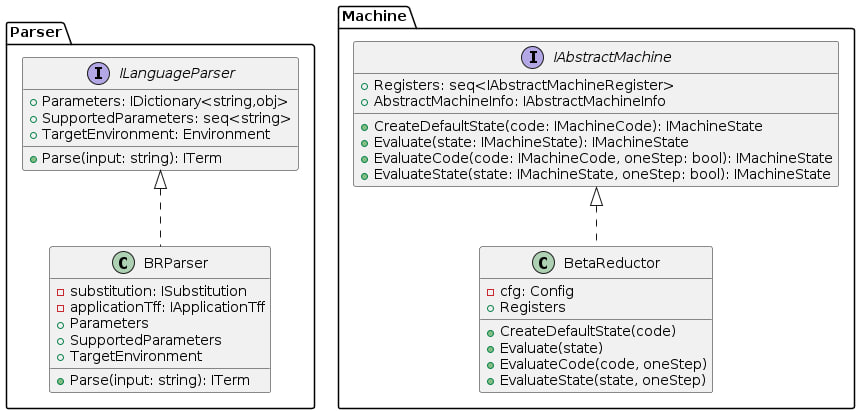
\includegraphics[width=0.8\textwidth]{./img/IAbstract.jpg}
  \caption{ILanguageParser и его реализация BRParser, а также IAbstractMachine и реализация BetaReductor}
  \label{fig:IAbstract}
\end{figure}

\section{Комбинаторный подход к проектированию синтаксического анализатора}
\label{sec:parser-api}

Синтаксический анализатор лямбда‑выражений представляет собой один из наиболее гибких компонентов системы. Его задача — преобразование текстового представления в абстрактное синтаксическое дерево (AST), пригодное для редукции и трансформаций. Особенностью реализованного решения является использование \textbf{комбинаторного подхода}, при котором парсер собирается из элементарных компонентов динамически, в рантайме.

\subsection{Базовая технология: FParsec}

В качестве основы используется библиотека \texttt{FParsec} — мощный парсер-комбинатор для языка F\#. Комбинаторы FParsec позволяют описывать синтаксис декларативно, как композицию простейших парсеров, что делает структуру анализатора читаемой, расширяемой и легко настраиваемой.

\subsection{Архитектурная модель}

Ключевая идея проектирования — построение синтаксического анализатора как функции от параметров конфигурации. Парсер создаётся в рантайме на основе объекта \texttt{Config}, в котором задаются:

\begin{itemize}
  \item поддерживаемые операторы (с приоритетами и ассоциативностью);
  \item список ключевых слов и их интерпретация;
  \item правила построения абстракций и аппликаций (TFF-модули);
  \item колбэки токенизации.
\end{itemize}

Таким образом, сам парсер — это не жёстко зафиксированная структура, а \textbf{генератор парсеров}, принимающий \texttt{Config} и возвращающий полностью настроенный объект для анализа конкретного языка.

\subsection{Конфигурация и расширяемость}

Конфигурация \texttt{Config} (рис. \ref{fig:config}) играет роль DSL для описания синтаксиса. Она включает:

\begin{itemize}
  \item \textbf{Операторы} — как унарные, так и бинарные, задаются в виде списка структур с полями: \texttt{keyword}, \texttt{term}, \texttt{priority}, \texttt{associativity}. Это позволяет реализовать приоритетный парсинг по методике Pratt Parser.
  \item \textbf{TFF-компоненты} — модули \texttt{simpleLambdaTff}, \texttt{applicationTff} управляют тем, как именно строится дерево термов (например, можно выбрать левостороннюю или правостороннюю аппликацию).
  \item \textbf{Ключевые слова и литералы} — список зарезервированных слов и способы их интерпретации. Например, \texttt{true}, \texttt{false}, \texttt{Y} транслируются в соответствующие комбинаторы.
\end{itemize}

\subsection{Колбэки и семантические действия}

Каждое правило разбора сопровождается соответствующим семантическим колбэком:

\begin{itemize}
  \item \texttt{brVarCallback(name)} — создаёт переменные;
  \item \texttt{brNumbersCallback(n)} — обрабатывает числовые литералы с типизацией;
  \item \texttt{brKeywordCallback(keyword)} — связывает ключевые слова с встроенными конструкциями.
\end{itemize}

Этот механизм позволяет адаптировать поведение парсера без изменения его ядра, что критически важно для реализации пользовательских языков и расширений.

\subsection{Интеграция с остальной системой}

Парсер BRParser реализует интерфейс \texttt{ILanguageParser}, предоставляя универсальный метод:

\begin{itemize}
  \item \texttt{Parse(input : string) : ITerm} — преобразует строку в AST;
  \item \texttt{Parameters} — управляют опциональными фичами (включение булевых литералов, допуск свободных переменных и пр.);
  \item \texttt{TargetEnvironment} — задаёт окружение, в котором происходит синтаксический анализ.
\end{itemize}

Таким образом, \texttt{BRParser} является не просто парсером, а обобщённым интерфейсом между текстовым представлением и термовым ядром вычислений.

\subsection{Обработка ошибок}

Обработка ошибок реализована в едином стиле: все исключения оборачиваются в тип \texttt{BRParsingException}, который:

\begin{itemize}
  \item сохраняет информацию о позиции и фрагменте ввода;
  \item предоставляет читаемое сообщение для отображения пользователю;
  \item хранит стек вызовов для внутренней отладки.
\end{itemize}

\begin{figure}[h]
  \centering
  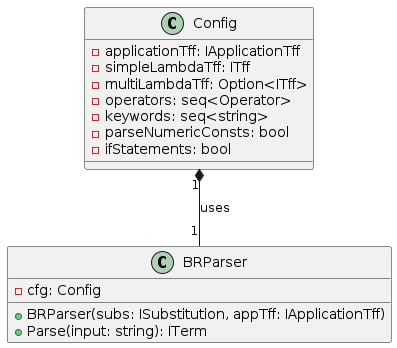
\includegraphics[width=0.8\textwidth]{./img/Config.jpg}
  \caption{Работа BRParser с Config}
  \label{fig:config}
\end{figure}


\section{Выводы}

В результате проектирования были получены:
\begin{itemize}
  \item Открытая модульная архитектура с работой через интерфейсы, позволившая легко расширять систему новыми компонентами;
  \item Полноценный API для абстрактной машины пошаговой бета‑редукции, поддерживающий как поэтапное, так и полное вычисление;
  \item Гибкий и настраиваемый API парсера, способный обрабатывать произвольные расширения синтаксиса, покрытый модульными тестами.
\end{itemize}

Эти результаты обеспечили надёжную основу для дальнейшей разработки и интеграции исследовательских и учебных сценариев работы с лямбда‑исчислением на платформе .NET.
